\documentclass{article}
\usepackage{amsrefs}
\usepackage{amssymb}
\usepackage{enumerate}
\usepackage{amsmath}
\usepackage{amsthm}
\usepackage{graphicx}
\usepackage{amssymb,latexsym}
\usepackage{graphicx}

\begin{document}

\begin{enumerate}

\item
\hfill

\begin{figure}[h]
\begin{center}
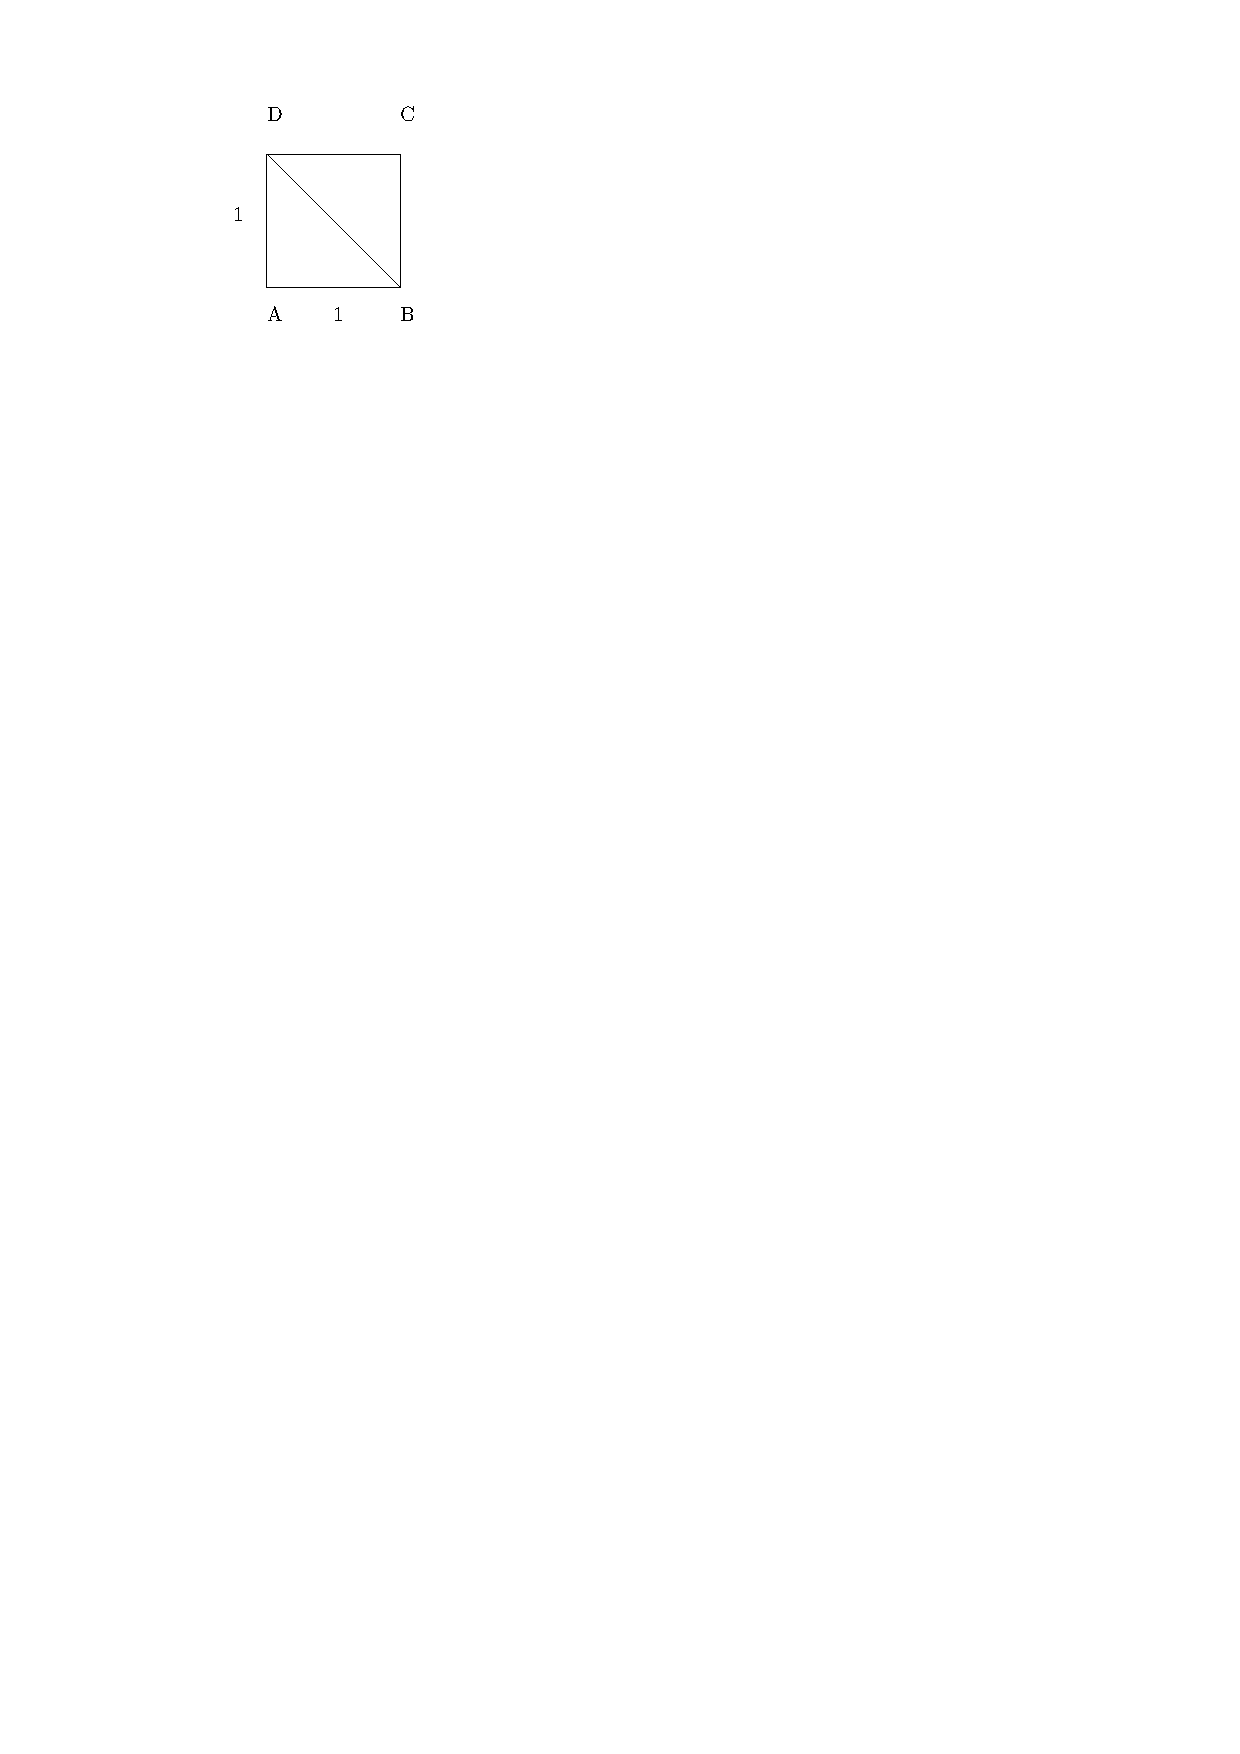
\includegraphics[height=4 cm]{TestOppInhoud1.pdf}
\caption{figuur bij opgave 1}
\end{center}
\end{figure}

In rechthoekige driehoek $ABD$ gebruik je de stelling van Pythagoras:
\[
\vert BD \vert ^2 = \vert AD \vert ^2 + \vert AB \vert ^2=1+1=2 \text { .}
\]
Je bekomt
\[
\vert BD \vert = \sqrt {2} \approx 1,41 \text {.}
\]

\item
\hfill

\begin{figure}[h]
\begin{center}
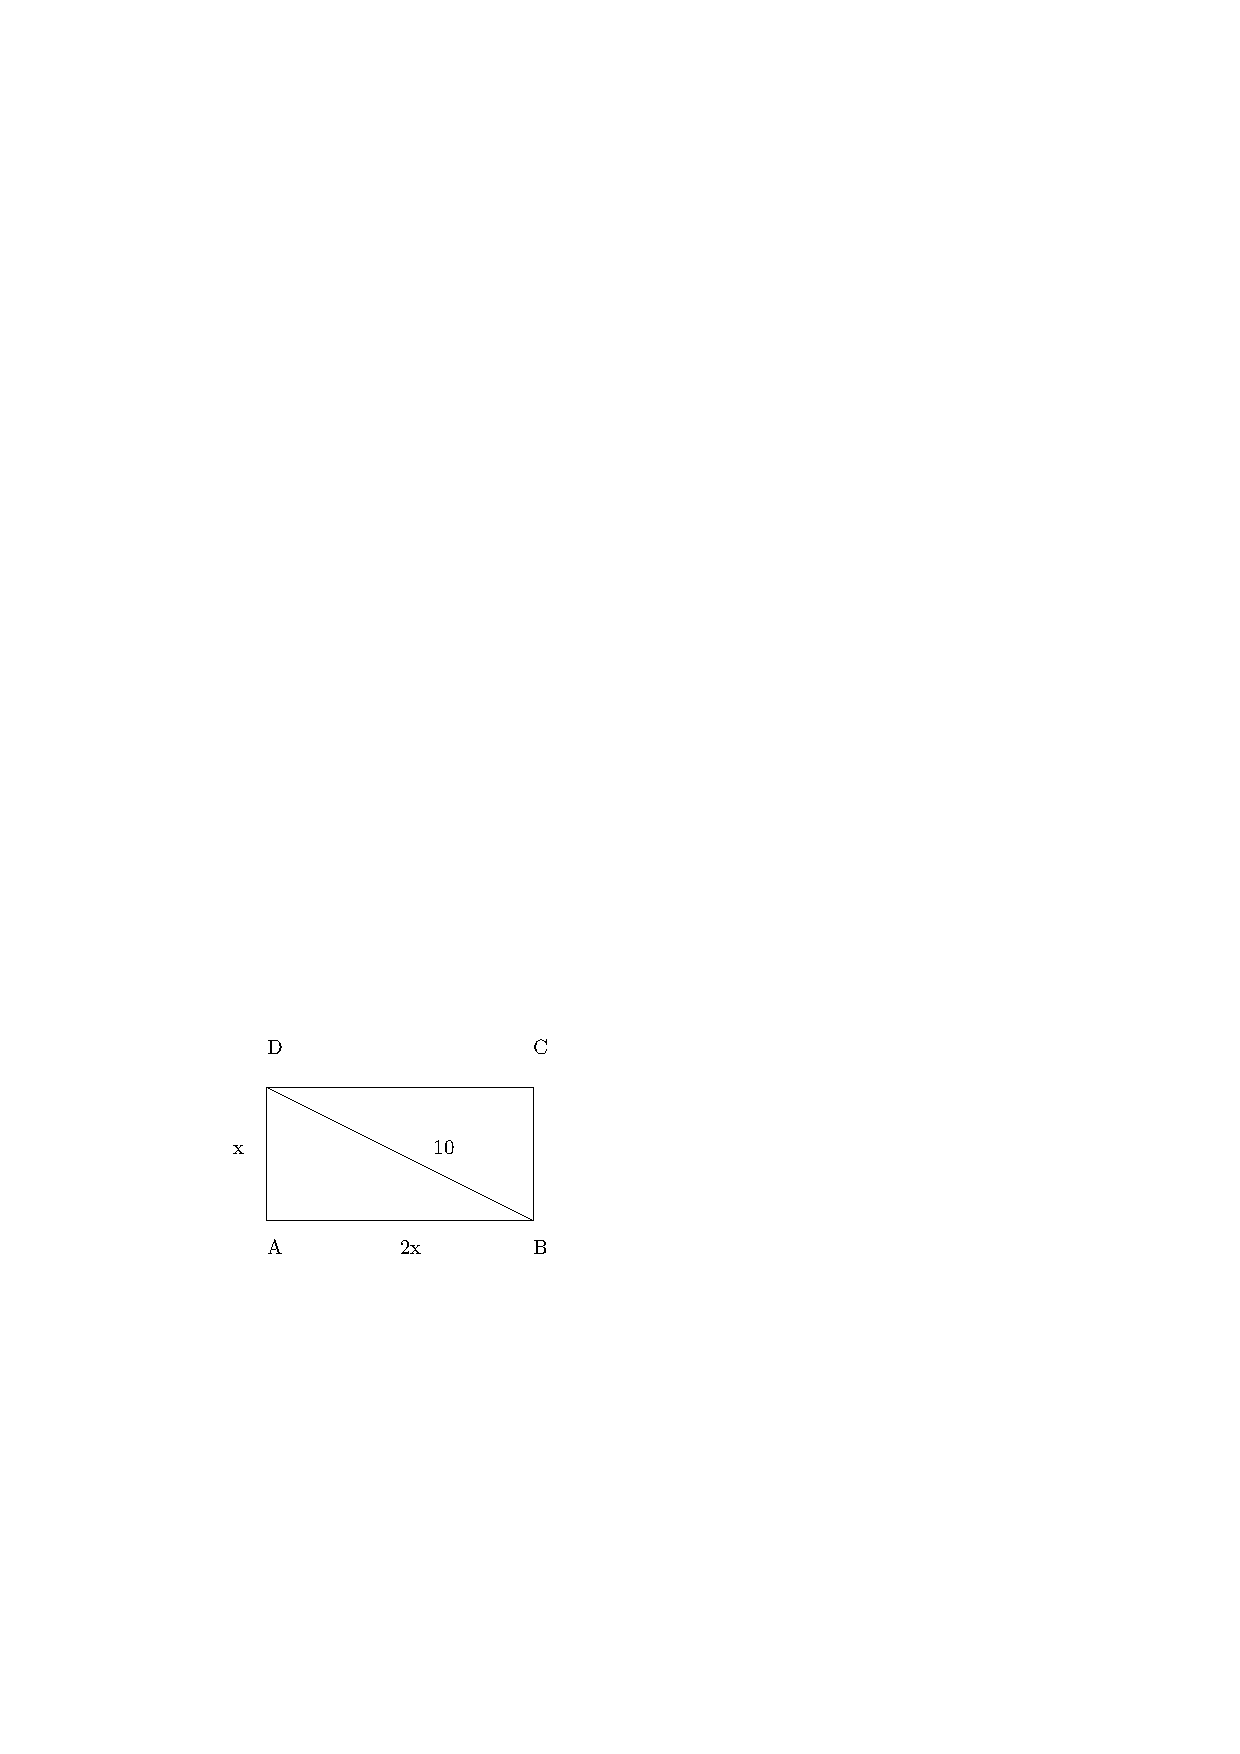
\includegraphics[height=4 cm]{TestOppInhoud2.pdf}
\caption{figuur bij opgave 2}
\end{center}
\end{figure}

De korte zijde heeft lengte $x$; de lange zijde heeft lengte $2x$.

In rechthoekige driehoek $ABD$ gebruik je de Stelling van Pythagoras:
\[
\vert AD \vert ^2+\vert AB \vert ^2= \vert BD \vert ^2
\]
dus
\[
x^2 +(2x)^2=10^2 \text { of } 5x^2=100 \text {; } x^2=20 \text { .}
\]

Je bekomt $x=\sqrt{20}$

De korte zijde $b$ heeft lengte $\sqrt {20} \approx 4,40$; de lange zijde $a$ heeft lengte $2\sqrt {20} \approx 8,94$.

\item

De straal van de aarde stellen we $x$ m.
De omtrek is dan $2 \pi x$ m (dit is 40000000 m).

Til het touw overal 1 m boven de grond dan wordt de straal $x+1$ m en de omtrek $2 \pi (x+1)$ m.

De omtrek neemt dus toe met $2 \pi$ m $\approx 6,28$ m.

\item
\hfill

\begin{figure}[h]
\begin{center}
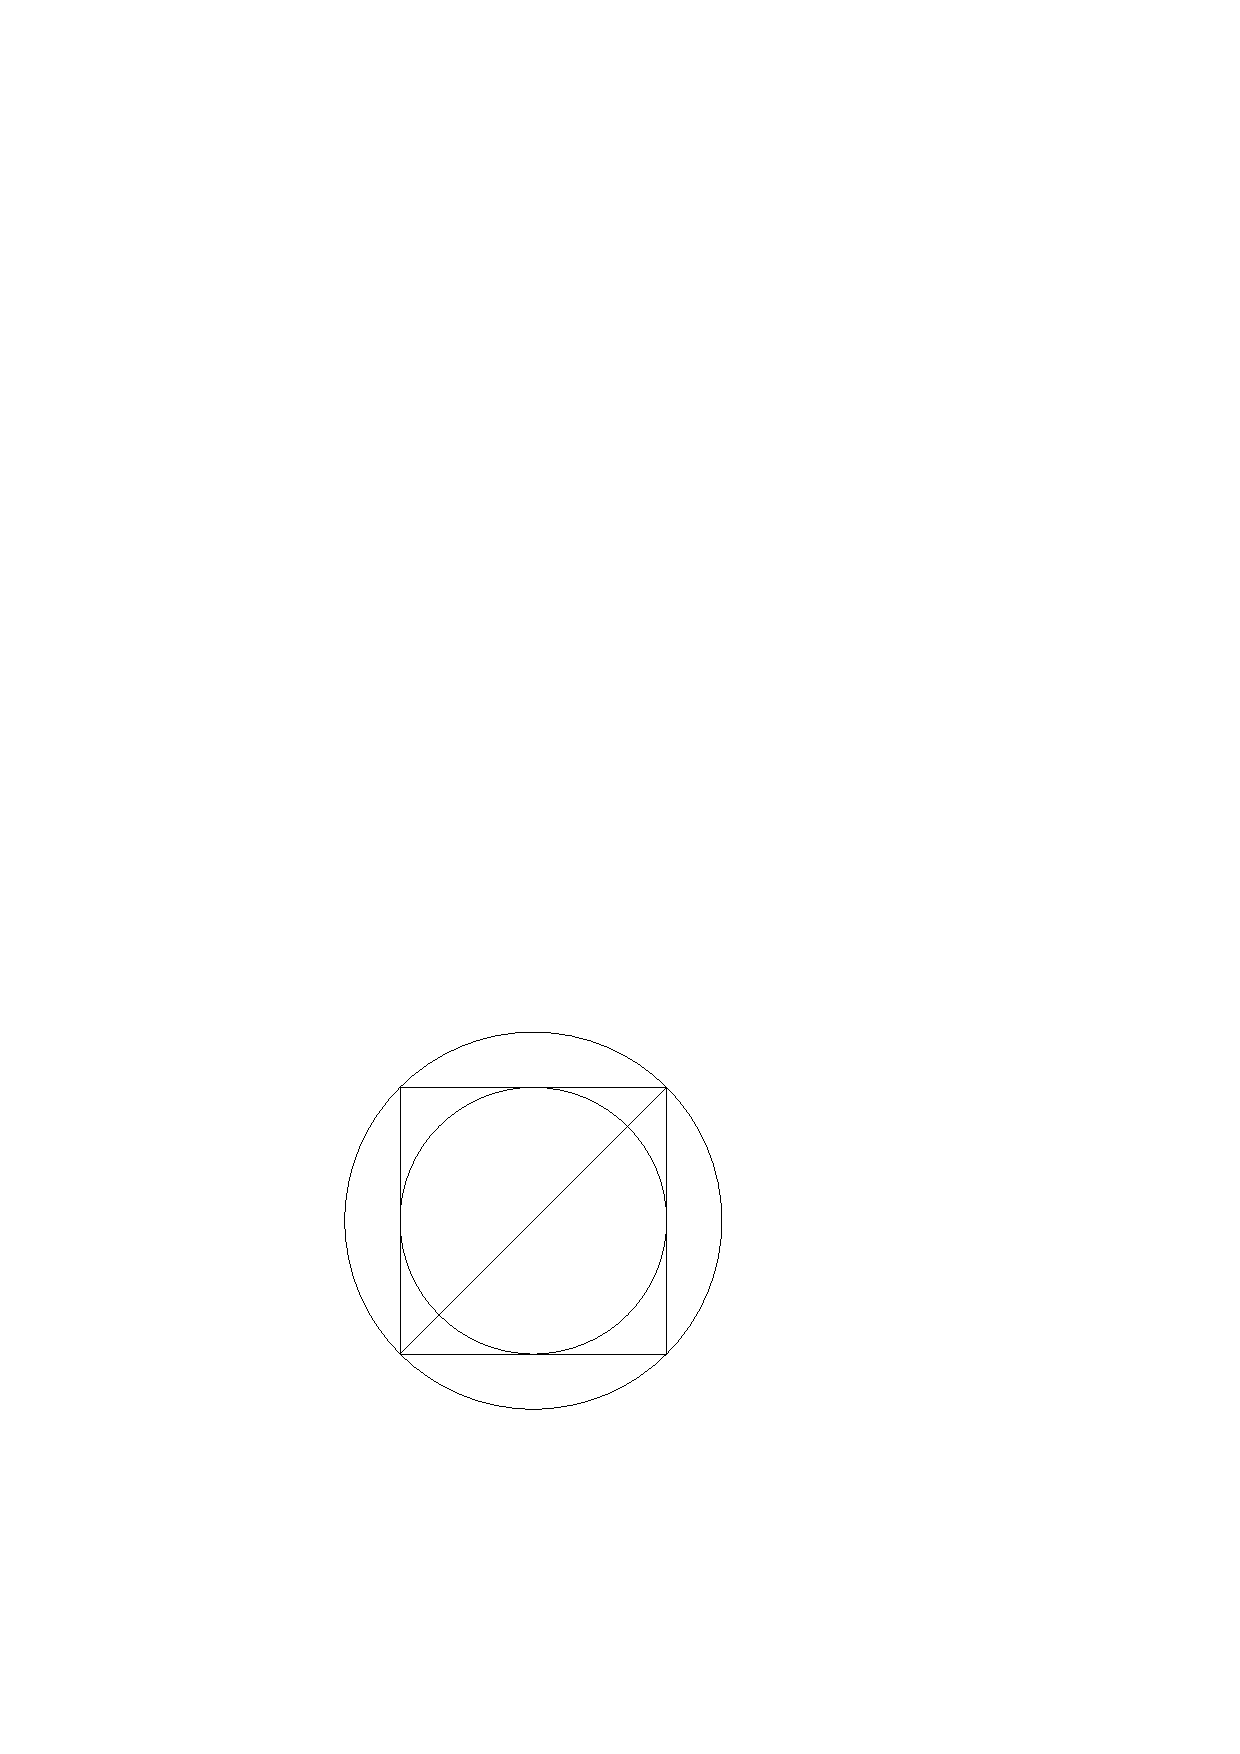
\includegraphics[height=4 cm]{TestOppInhoud4.pdf}
\caption{figuur bij opgave 4}
\end{center}
\end{figure}

De lengte van de zijde van het vierkant noteren we met $z$.

De straal van de ingeschreven cirkel is gelijk aan $\frac{z}{2}$ en de oppervlakte van de ingeschreven cirkel is daarom $\pi \left( \frac{z}{2} \right)^2=\frac {\pi z^2}{4}$.

De straal van de omgeschreven cirkel is gelijk aan de helft van de lengte van de diagonaal van het vierkant.
De lengte van zulke diagonaal is $\sqrt{2} z$ (zie de oplossing bij opgave 1 uit deze reeks).
De straal van de omgeschreven cirkel is dus $\frac{\sqrt{2}z}{2}$ en de oppervlakte van de omgeschreven cirkel is daarom $\pi \left( \frac {z}{\sqrt{2}} \right)^2=\frac {\pi z^2}{2}$.

De gevraagde verhouding is dus $\frac {\frac{\pi z^2}{2}}{\frac {\pi z^2}{4}}=2$.

\item

Om juist te zijn moeten de 3 vergelijkingen gelden en dat is zo.

\item

De oppervlakte van het grondvlak is $\frac{120.154}{2} cm^2=9240 cm^2$.

Het volume van de bloembak is dus $9240.35 cm^3=323400 cm^3$.

Omdat $1 dm^3=1000 cm^3$ bekom je als volume voor de bloembak $323,40 dm^3$.

\item

Het vooraanzicht verdelen we in twee delen:

\begin{figure}[h]
\begin{center}
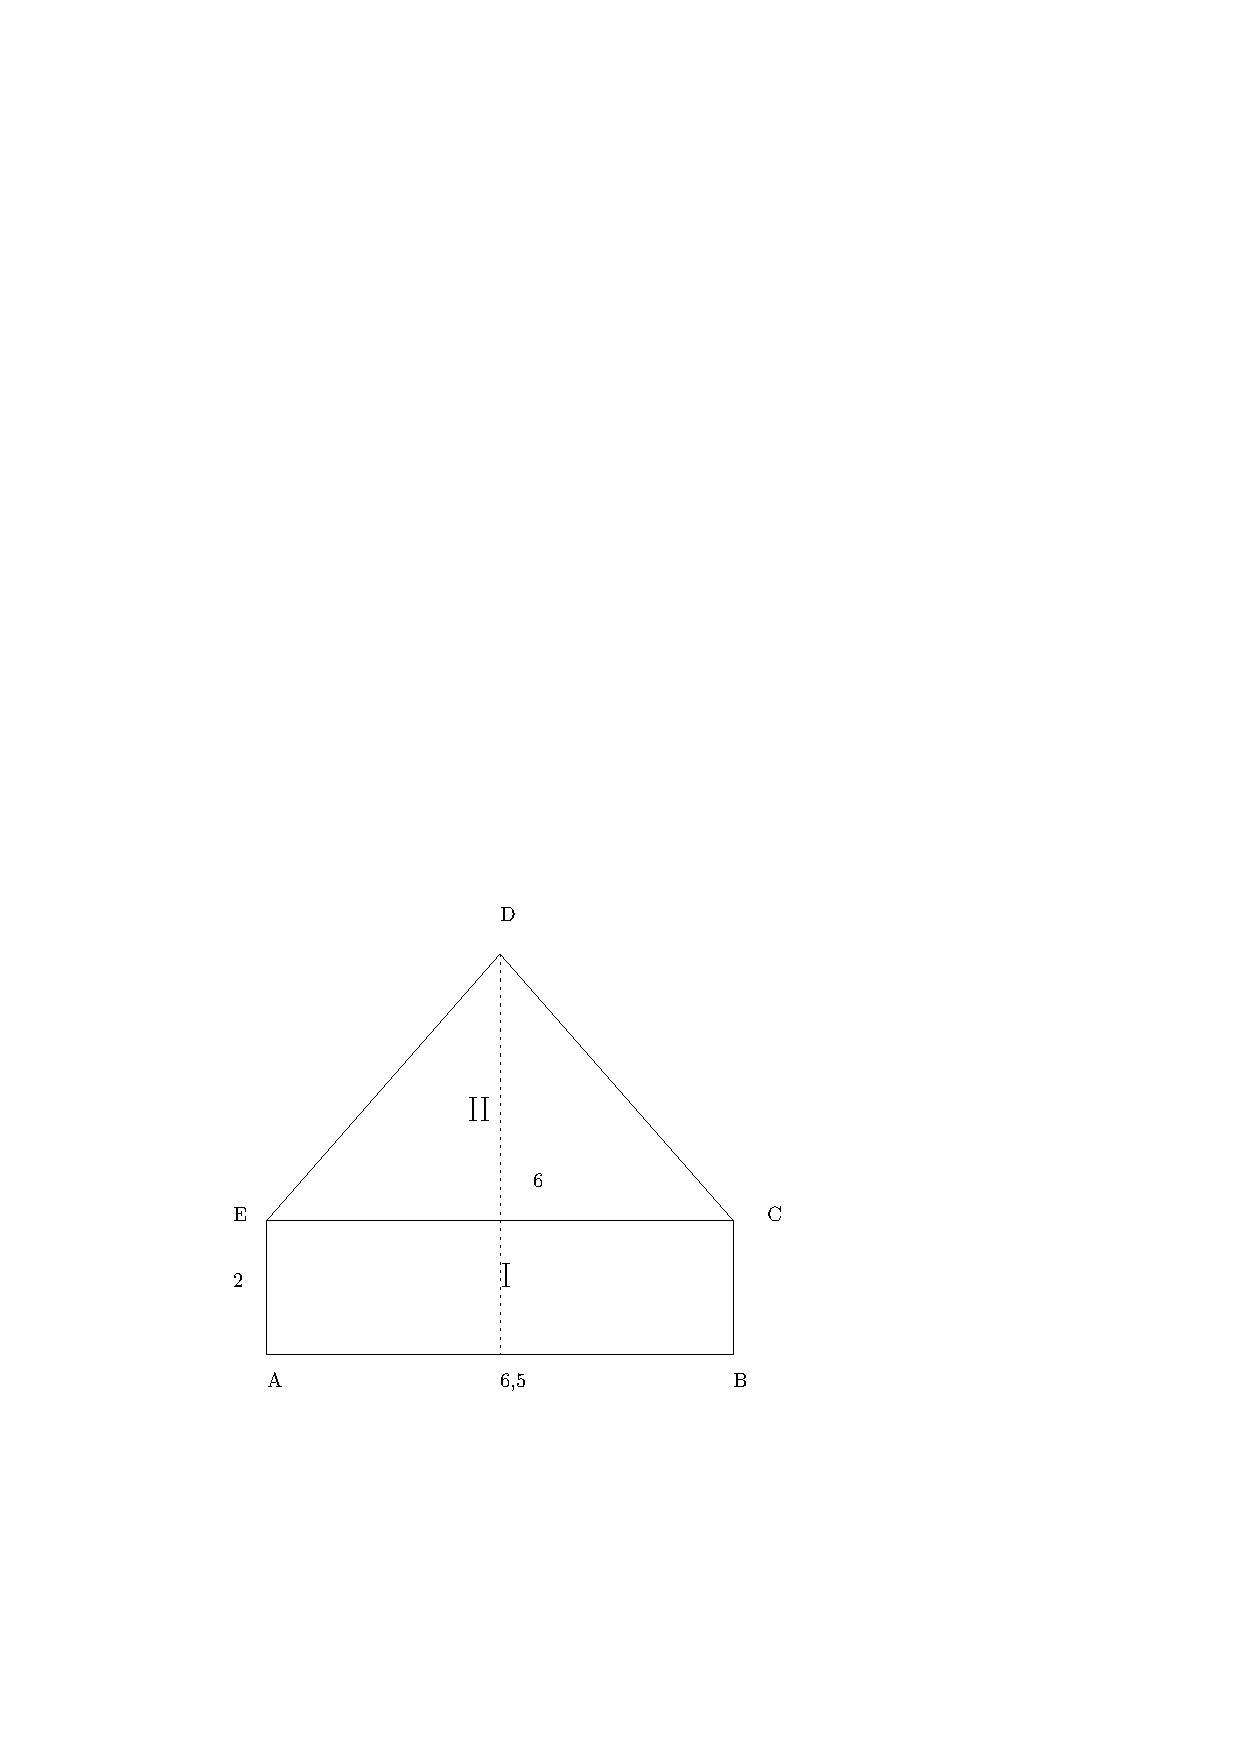
\includegraphics[height=5 cm]{TestOppInhoud7.pdf}
\caption{figuur bij opgave 7}
\end{center}
\end{figure}

Omdat $D$ op hoogte 6 m boven $AB$ is, is de hoogte van driehoek $ECD$ gelijk aan $(6-2) m = 4 m$.

De oppervlakte van deel I is $6,5.2 m^2=13 m^2$ en de oppervlakte van deel II is $\frac{6,5.4}{2} m^2=13 m^2$.

Rekening houdend met de constante diepte 5 m bekom je als volume
\[
(13+13).5 m^3 = 130 m^3 \text { .}
\]

\item

De Grote Piramide heeft als grondvlak een vierkant.
De oppervlakte van dat vierkant is $230^2 m^2=52900 m2$.

Het volume van de Grote Piramide is dus $\frac{1}{3} . 52900.146 m^3=2574466,667 m^3$.

Er worden ongeveer 2300000 blokken gebruikt; ieder blok heeft dan volume $\frac{2574466,667}{2300000} m^3 = 1,12 m^3$.

\item

Het volume van zulke bolvormige kaars is $\frac{4}{3}.\pi.4^3 cm^3=268,08 cm^3$.

Omdat $1 l$ kaarsvet $= 1 dm^3$ kaarsvet $= 1000 cm^3$ kaarsvet en $\frac{1000}{268,08}=3,73$ bekom je dat 3 volledige zulke bolvormige kaarsen kunnen gemaakt worden.

\item

We noteren $R$ mm voor de straal van zulke tennisbal.

Dan is $6R=195$, dus $R=\frac{195}{6}=32,5$.

Het volume van zulke tennisbal is dus $\frac{4}{3} 32,5^3 mm^3=143793,3137 mm^3$.

Het volume van de koker (oppervalkte grondvlak.hoogte) is $\pi .32,5^2.195 mm^3=647069,9119 mm^3$.

Het resterende volume in de koker is daarom
\[
647069,9119 mm^3 - 3.143793,3137 mm^3=215689,970 mm^3 \approx 215,69 cm^3 \text { .}
\]

\item

Het volume van het glas is $\frac{1}{3} . \pi . 5,5^2.9 cm^3=285,099533 cm^3$.

Zulk glas wordt gevuld met $0,9.285,099533 cm^3 = 256,58958 cm^3$.

In totaal is er $10 dm^3=10000 cm^3$ wijn.
Omdat $\frac{10000}{256,58958}=38,97$ kun je aan 38 genodigden een gevuld glas geven.

\end{enumerate}

\end{document}